\chapter{T-дуальность, D-браны и калибровочная теория}

\lectureoverview{T-дуальность начинается как точная эквивалентность между замкнутыми струнами на окружностях радиусов (R) и \(\alpha'/R\). Импульс и намотка меняются ролями, как и производные по мировому листу \(\partial_\tau Y\) и \(\partial_\sigma Y\), а также пространственно-временные векторы, происходящие из \(G_{\mu 5}\) и \(B_{\mu 5}\). Когда та же операция применяется к открытой струне, граничное условие Неймана на конце превращается в условие Дирихле. Тогда конец должен лежать на динамической D-бране. Открытые струны, ограниченные одной браной, при низких энергиях дают абелеву калибровочную теорию; струны, соединяющие стопку бран, несут две метки концов и дают неабелеву калибровочную теорию. D-струна, оканчивающаяся на D3-бране, дает соответствующий магнитный монополь.}

\section{Почему мы возвращаемся к T-дуальности?}

Мы уже встречались с T-дуальностью, но возвращаемся к ней не случайно. Она была одной из подсказок того, что теория струн содержит гораздо больше, чем возмущательные струны. Когда были поняты ее следствия для открытых струн, это привело к D-бранам; D-браны, в свою очередь, стали способом строить и изучать квантовые теории поля. Поэтому цель этой лекции состоит не просто в том, чтобы повторить лозунг о том, что малая окружность эквивалентна большой. Мы достаточно тщательно заново выстроим рассуждение, чтобы увидеть, как этот лозунг вынуждает появиться в теории новым физическим объектам.

Простейшая постановка — тороидальная компактификация. Одномерный тор — это окружность. Двумерный тор можно представить параллелограммом, у которого отождествлены противоположные стороны, а трехмерный тор — параллелепипедом с отождествленными противоположными гранями. Та же конструкция продолжается и в более высоких измерениях. Мы оставим только одну компактную пространственную координату, обозначаемую \(Y\), и одну типичную некомпактную координату, обозначаемую \(X\). Время присутствует, но на рисунках на доске не показано.

Выберем стандартное соглашение
\begin{equation}
  Y\sim Y+2\pi R,
  \label{eq:l10-circle-identification}
\end{equation}
так что \(R\) — это радиус, а \(2\pi R\) — длина окружности. В лекции компактный размер часто обозначается просто \(r\) и опускаются множители \(2\pi\) и \(\alpha'\). В выводах мы сохраним стандартные множители и будем указывать единицы, используемые в лекции, когда это полезно.

В первой половине обсуждения струны замкнутые и ориентированные. Ориентация — это внутренняя стрелка, проведенная вдоль струны. Если всюду обратить все стрелки, ни один эксперимент не изменится; важна относительная ориентация двух струн. При расщеплении и соединении стрелки должны соединяться непрерывно. Это первый намек на то, что появится сохраняющаяся величина со знаком.

\begin{figure}[H]
  \centering
  \includegraphics[width=0.72\textwidth]{lecture_10_figure_01.png}
  \caption{Две замкнутые струны с отмеченными на доске их относительными ориентациями. При расщеплении и соединении ориентация должна оставаться непрерывной.}
  \lectureframe{00:05:40}
  \label{fig:l10-oriented-closed-strings}
\end{figure}

\begin{classroomqa}
\audiencequestion{Если координата мирового листа пробегает от \(\sigma=0\) до \(2\pi\), значит ли это, что струна уже один раз обошла компактное направление? \lecturetimestamp{00:08:42}}
\lecturerresponse{Нет. Координата \(\sigma\) помечает точки вдоль струны; она не задает положения в компактном пространстве. У любой замкнутой струны есть периодический параметр \(\sigma\), независимо от того, намотана она или нет. Полезна аналогия с резиновым кольцом: можно пронумеровать молекулы по окружности резинового кольца, даже если оно ни на что не намотано. Намотка — это свойство отображения \(Y(\tau,\sigma)\), а не одного лишь параметра \(\sigma\).}
\end{classroomqa}

\begin{classroomqa}
\audiencequestion{Должен ли компактный размер также быть одинаковым при каждом значении большой координаты \(X\)? \lecturetimestamp{00:10:00}}
\lecturerresponse{Необязательно при общей динамической компактификации. Мы начинаем с фиксированной окружности, потому что это самый чистый фон. Позже компонента \(G_{55}\) станет скалярным полем, значение которого измеряет локальный размер пятого направления, так что этот размер может меняться по обычному пространству-времени.}
\end{classroomqa}

\section{Намотка сохраняется даже при пересоединении струн}

Ненамотанная струна может двигаться через компактное направление, не охватывая его. Намотанная струна устроена иначе: когда \(\sigma\) один раз обходит замкнутую струну, вложение \(Y(\tau,\sigma)\) проходит через один или несколько периодов компактной окружности. Поскольку струна ориентирована, это продвижение имеет знак. Струна может наматываться в положительном или в отрицательном направлении.

Закон сохранения яснее всего виден на рисунках соединения. Возьмем одну струну с намоткой \(+1\) и другую с намоткой \(-1\). Их совместимые участки могут пересоединиться. Получающаяся конфигурация имеет нулевую суммарную намотку и может быть деформирована в ненамотанную струну. На доске прослежено именно такое пересоединение для противоположных ориентаций.

\begin{figure}[H]
  \centering
  \includegraphics[width=0.72\textwidth]{lecture_10_figure_02.png}
  \medskip

  \begin{tikzpicture}[x=1cm,y=1cm,>=Latex]
    \draw[thick] (-4.0,0.3) circle (0.65);
    \draw[->,thick] (-4.55,0.58) arc (150:-145:0.65);
    \node at (-4.0,-0.65) {$w=+1$};
    \draw[thick] (-2.0,0.3) circle (0.65);
    \draw[<-,thick] (-2.55,0.58) arc (150:-145:0.65);
    \node at (-2.0,-0.65) {$w=-1$};
    \node at (-3.0,0.3) {$+$};
    \draw[->,thick] (-1.0,0.3) -- (0.3,0.3);
    \draw[thick] (1.4,0.3) ellipse (0.95 and 0.55);
    \node at (1.4,-0.65) {$w_{\rm total}=0$};
  \end{tikzpicture}
  \caption{Намотки противоположных знаков пересоединяются в конфигурацию с нулевой суммарной намоткой. Нижняя диаграмма — это аккуратная реконструкция хода на доске, а не второй динамический процесс.}
  \lectureframe{00:13:20}
  \label{fig:l10-opposite-winding}
\end{figure}

Теперь повторим эксперимент с двумя струнами одинаковой ориентации. Они могут соединиться, но не могут размотаться. Результат несет намотку, вдвое большую, чем у любой из входящих струн. Число отдельных связных струн изменилось; полная намотка — нет.

\begin{figure}[H]
  \centering
  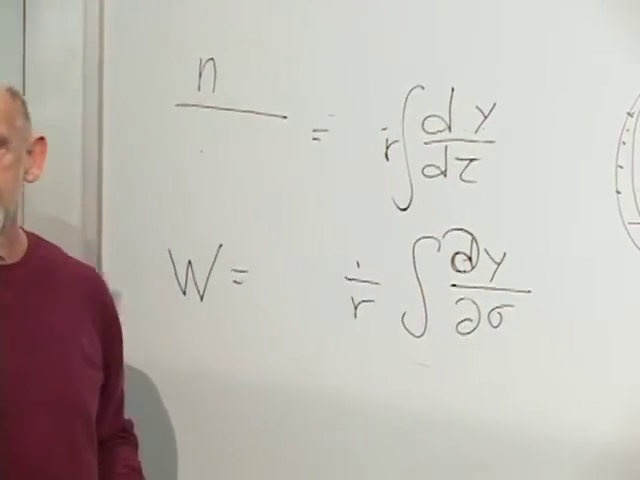
\includegraphics[width=0.72\textwidth]{lecture_10_figure_03.png}
  \medskip

  \begin{tikzpicture}[x=1cm,y=1cm,>=Latex]
    \draw[thick] (-4.0,0.3) circle (0.65);
    \draw[->,thick] (-4.55,0.58) arc (150:-145:0.65);
    \node at (-4.0,-0.65) {$w=+1$};
    \draw[thick] (-2.0,0.3) circle (0.65);
    \draw[->,thick] (-2.55,0.58) arc (150:-145:0.65);
    \node at (-2.0,-0.65) {$w=+1$};
    \node at (-3.0,0.3) {$+$};
    \draw[->,thick] (-1.0,0.3) -- (0.3,0.3);
    \draw[thick] (1.45,0.3) circle (0.78);
    \draw[thick] (1.45,0.3) circle (0.52);
    \draw[->,thick] (0.81,0.74) arc (145:-145:0.78);
    \node at (1.45,-0.78) {$w=+2$};
  \end{tikzpicture}
  \caption{Намотки одного знака могут пересоединиться в дважды намотанную струну. Связность меняется, тогда как полная намотка остается равной двум.}
  \lectureframe{00:16:40}
  \label{fig:l10-same-winding}
\end{figure}

Это различие сохраняется при любом допустимом процессе. Полная намотка величиной сто может переноситься одной струной, намотанной сто раз, двумя струнами, каждая из которых намотана пятьдесят раз, или ста однократно намотанными струнами. Струны могут расщепляться и соединяться, переходя между этими описаниями, но знаковая сумма остается равной ста. Мы обозначаем ее через \(w\in\mathbb Z\).

\section{Моды импульса и моды намотки}

Само по себе сохранение еще не является дуальностью. Теперь сравним энергии. Состояние, движущееся по компактной окружности, имеет квантованный импульс
\begin{equation}
  p_Y=\frac{n}{R},
  \qquad n\in\mathbb Z.
  \label{eq:l10-compact-momentum}
\end{equation}
Для состояния, у которого остальными вкладами в массу можно пренебречь, компактное движение дает вклад \(E_{\rm mom}=|n|/R\). Положительные и отрицательные \(n\) обозначают противоположные направления движения, тогда как энергия положительна.

\begin{figure}[H]
  \centering
  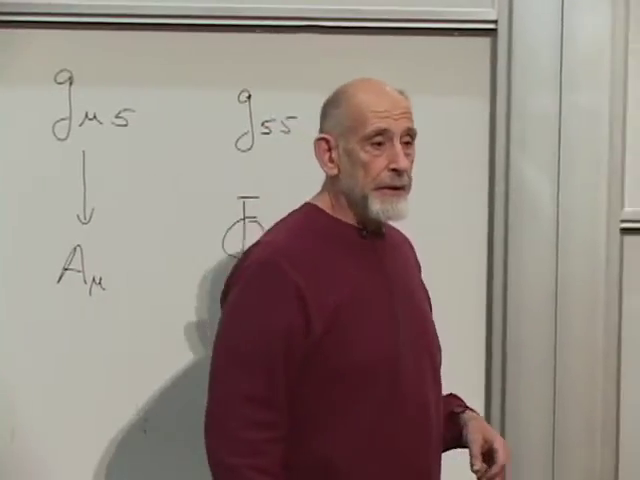
\includegraphics[width=0.72\textwidth]{lecture_10_figure_04.png}
  \caption{Квантовое число компактного импульса на доске. В лекции импульс схематически записывается как интеграл от компактной скорости.}
  \lectureframe{00:21:30}
  \label{fig:l10-compact-momentum-board}
\end{figure}

Струна, намотанная \(|w|\) раз, имеет длину \(2\pi |w|R\). При натяжении фундаментальной струны
\begin{equation}
  T_{\rm F}=\frac{1}{2\pi\alpha'},
\end{equation}
ее энергия намотки равна
\begin{equation}
  E_{\rm wind}=T_{\rm F}(2\pi |w|R)
  =\frac{|w|R}{\alpha'}.
  \label{eq:l10-winding-energy}
\end{equation}
В единицах лекции \(\alpha'=1\) это просто \(E_{\rm wind}=|w|R\).

Эти две башни при изменении радиуса ведут себя противоположным образом. При \(R\gg
\sqrt{\alpha'}\) уровни импульса расположены тесно, а уровни намотки — редко. При \(R\ll\sqrt{\alpha'}\) уровни импульса расположены редко, а уровни намотки — тесно.

\begin{figure}[H]
  \centering
  \begin{minipage}[t]{0.48\textwidth}
    \centering
    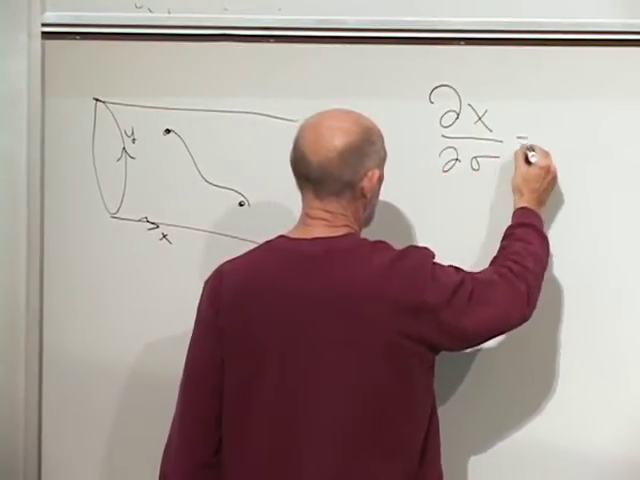
\includegraphics[width=\linewidth]{lecture_10_figure_05.png}
    \par\smallskip
    \textit{Большой компактный радиус.}
  \end{minipage}\hfill
  \begin{minipage}[t]{0.48\textwidth}
    \centering
    \includegraphics[width=\linewidth]{lecture_10_figure_06.png}
    \par\smallskip
    \textit{Малый компактный радиус.}
  \end{minipage}
  \caption{Два спектральных сравнения на доске. При обращении радиуса разреженные и плотные башни меняются ролями.}
  \lectureframe{00:25:30--00:26:00}
  \label{fig:l10-dual-spectra-board}
\end{figure}

Наглядная схема такова:
\begin{figure}[H]
  \centering
  \begin{adjustbox}{max width=\linewidth}
  \begin{tikzpicture}[x=1cm,y=0.74cm,>=Latex]
    \node[font=\bfseries] at (-3.6,6.2) {$R\gg\sqrt{\alpha'}$};
    \draw[->] (-5.1,0) -- (-5.1,5.5) node[above] {$E$};
    \foreach \y in {0.4,1.0,1.6,2.2,2.8,3.4,4.0,4.6}
      \draw (-5.35,\y)--(-4.85,\y);
    \node[align=center] at (-4.25,5.15) {momentum\\dense};
    \draw[->] (-2.2,0) -- (-2.2,5.5) node[above] {$E$};
    \foreach \y in {0.4,2.4,4.4}
      \draw (-2.45,\y)--(-1.95,\y);
    \node[align=center] at (-1.35,5.15) {winding\\sparse};

    \node[font=\bfseries] at (3.6,6.2) {$R\ll\sqrt{\alpha'}$};
    \draw[->] (2.2,0) -- (2.2,5.5) node[above] {$E$};
    \foreach \y in {0.4,2.4,4.4}
      \draw (1.95,\y)--(2.45,\y);
    \node[align=center] at (3.05,5.15) {momentum\\sparse};
    \draw[->] (5.1,0) -- (5.1,5.5) node[above] {$E$};
    \foreach \y in {0.4,1.0,1.6,2.2,2.8,3.4,4.0,4.6}
      \draw (4.85,\y)--(5.35,\y);
    \node[align=center] at (5.95,5.15) {winding\\dense};
  \end{tikzpicture}
  \end{adjustbox}
  \caption{Реконструкция аргумента о расстояниях между уровнями. Полный спектр струн не изменяется при обмене импульса и намотки вместе с \(R\leftrightarrow\alpha'/R\).}
  \label{fig:l10-dual-spectra-redraw}
\end{figure}

Предположим, наблюдателю дают один из этих спектров, не сообщая, как он был получен. Является ли тесно расположенная башня импульсом на большой окружности или намоткой на малой? По одному спектру этого сказать нельзя. Теория струн делает более сильное утверждение: амплитуды рассеяния тоже не могут этого различить. Эти два описания в точности эквивалентны при
\begin{equation}
  n\longleftrightarrow w,
  \qquad
  R\longleftrightarrow \widetilde R=\frac{\alpha'}{R}.
  \label{eq:l10-radius-duality}
\end{equation}
Неподвижная точка равна
\begin{equation}
  R=\sqrt{\alpha'},
  \label{eq:l10-self-dual-radius}
\end{equation}
или \(R=1\) в единицах лекции. При этом радиусе дополнительные состояния могут стать безмассовыми, а калибровочная симметрия усиливается.

\begin{classroomqa}
\audiencequestion{Является ли намотка лишь математическим удобством для переписывания спектра? \lecturetimestamp{00:27:33}}
\lecturerresponse{Нет. Намотка обозначает реальные сектора гильбертова пространства замкнутой струны, и эти секторы участвуют во взаимодействиях. Слово ``дуальность'' означает, что описание через импульс и описание через намотку — это разные координаты одной и той же физики, а не то, что один сектор служит необязательным мнемоническим приемом для другого.}
\end{classroomqa}

\begin{classroomqa}
\audiencequestion{Существует ли радиус, который отображается сам в себя?
\lecturetimestamp{00:27:58}}
\lecturerresponse{Да. Самодуальное значение равно \(R=\sqrt{\alpha'}\), что составляет \(R=1\) в единицах, использованных на доске. Там две башни встречаются, и спектр обладает усиленной симметрией.}
\end{classroomqa}

\section{Форма дуальности на мировом листе}

Спектральный аргумент наводит на эту мысль, но описание на мировом листе делает обмен более точным. В конформной калибровке импульс, сопряженный \(Y\), пропорционален \(\partial_\tau Y\). Поэтому суммарный импульс вдоль компактного направления имеет вид
\begin{equation}
  P_Y=\frac{1}{2\pi\alpha'}
      \int_0^{2\pi}d\sigma\,\partial_\tau Y.
  \label{eq:l10-worldsheet-momentum}
\end{equation}
Число намотки равно
\begin{equation}
  w=\frac{1}{2\pi R}
      \int_0^{2\pi}d\sigma\,\partial_\sigma Y
   =\frac{Y(2\pi)-Y(0)}{2\pi R}.
  \label{eq:l10-worldsheet-winding}
\end{equation}

\begin{classroomqa}
\audiencequestion{Почему интеграл от производной вдоль замкнутой струны не обращается в нуль? \lecturetimestamp{00:32:33}}
\lecturerresponse{Потому что \(Y\) — периодическая координата пространства-мишени, а не однозначная вещественная функция на \(\sigma\)-окружности. Точка мирового листа \(\sigma=2\pi\) совпадает с \(\sigma=0\), но подъём вложения на накрывающую прямую меняется на \(2\pi wR\). Интеграл от \(\partial_\sigma Y\) измеряет этот сдвиг.}
\end{classroomqa}

\begin{figure}[H]
  \centering
  \includegraphics[width=0.76\textwidth]{lecture_10_figure_07.png}
  \caption{Интегралы для импульса и намотки после того, как на доске дописаны обе строки. В лекционной нормировке общие множители \(2\pi\) и \(\alpha'\) опущены.}
  \lectureframe{00:33:25}
  \label{fig:l10-momentum-winding-integrals}
\end{figure}

Для струны с одной намоткой,
\begin{equation}
  Y(\tau,\sigma+2\pi)=Y(\tau,\sigma)+2\pi R.
\end{equation}
При намотке \(w\) сдвиг в правой части равен \(2\pi wR\). Тогда уравнение \eqref{eq:l10-worldsheet-winding} точно даёт число намотки. Это точная версия краткой записи на доске \(w\sim R^{-1}\int
d\sigma\,\partial_\sigma Y\).

Формулировка T-дуальности на мировом листе поэтому имеет вид
\begin{equation}
  \partial_\tau Y\longleftrightarrow
  \partial_\sigma \widetilde Y,
  \qquad
  \partial_\sigma Y\longleftrightarrow
  \partial_\tau \widetilde Y,
  \label{eq:l10-derivative-duality}
\end{equation}
при этом импульс по \(Y\) переходит в намотку по двойственной координате \(\widetilde Y\), и наоборот.

\begin{classroomqa}
\audiencequestion{Означает ли это, что сами координаты мирового листа \(\tau\) и \(\sigma\) связаны между собой или меняются местами?
\lecturetimestamp{00:34:39}}
\lecturerresponse{Нет. T-дуальность отображает решения друг в друга и обменивает определенные производные компактной координаты пространства-мишени. Она не отождествляет временную координату мирового листа с его пространственной координатой.}
\end{classroomqa}

\section{Почему состояний с намоткой нельзя избежать}

Можно спросить, почему струна вообще может оказаться в состоянии с намоткой, если доступно состояние без намотки. Струна не выбирает свое состояние по предпочтению. Энергия, сообщенная при столкновении, растягивает ее. Достаточно энергичная, сильно деформированная струна может в результате пересоединения превратиться в две струны с противоположной намоткой. Их суммарная намотка остается нулевой, но после расщепления две струны могут разойтись. Одну из пары можно унести далеко, оставив наблюдателю, по-видимому, изолированную намотанную струну.

\begin{figure}[H]
  \centering
  \includegraphics[width=0.76\textwidth]{lecture_10_figure_08.png}
  \caption{Сильно растянутая конфигурация с нулевой суммарной намоткой, из которой после пересоединения могут разойтись струны с противоположной намоткой.}
  \lectureframe{00:36:15}
  \label{fig:l10-winding-pair-production}
\end{figure}

Энергетический порог определяется энергией намотки. На большой окружности нужна большая энергия столкновения, чтобы обернуть вокруг компактного направления достаточно длинный участок струны. Однако выше порога нельзя запретить рождение пары намотка--антинамотка. Аналогия здесь — столкновения фотонов, порождающие электрон--позитронную пару. Полный электрический заряд по-прежнему равен нулю, однако заряженные частицы присутствуют и могут быть разделены. Сохранение намотки работает точно так же.

Эта аналогия не просто словесная. Компактный импульс и намотка ведут себя как два различных квантовых числа заряда. В соответствующем редуцированном описании одинаковые знаки отталкиваются, а противоположные притягиваются. Поэтому следует спросить, какие два векторных поля переносят эти силы.

\section{Импульсный заряд из пятимерной гравитации}

Начнем с гравитации в пяти измерениях. Пусть индексы \(M,N\) пробегают четыре обычных направления пространства-времени и компактное пятое направление. Метрика разлагается как
\begin{equation}
  G_{MN}\quad\longrightarrow\quad
  \bigl\{G_{\mu\nu},\,G_{\mu5},\,G_{55}\bigr\}.
  \label{eq:l10-metric-decomposition}
\end{equation}
Симметричная компонента \(G_{5\mu}\) не содержит никакой новой информации по сравнению с \(G_{\mu5}\).

\begin{figure}[H]
  \centering
  \includegraphics[width=0.74\textwidth]{lecture_10_figure_09.png}
  \caption{Независимые группы компонент пятимерной метрики: \(G_{\mu\nu}\), \(G_{\mu5}\) и \(G_{55}\).}
  \lectureframe{00:44:05}
  \label{fig:l10-metric-components}
\end{figure}

С четырехмерной точки зрения,
\begin{align}
  G_{\mu\nu} &\quad\hbox{is a spacetime metric},\\
  G_{\mu5} &\equiv A_\mu\quad\hbox{is a vector field},\\
  G_{55} &\equiv e^{2\varphi}\quad\hbox{is a scalar modulus}.
  \label{eq:l10-four-dimensional-fields}
\end{align}
Скаляр \(\varphi\) определяет размер компактного направления. Он может гладко меняться по обычному пространству-времени, так что волны \(\varphi\) — это волны радиуса пятого измерения.

\begin{figure}[H]
  \centering
  \includegraphics[width=0.74\textwidth]{lecture_10_figure_10.png}
  \caption{На доске \(G_{\mu5}\) отождествляется с вектором \(A_\mu\), а \(G_{55}\) — со скаляром \(\Phi\).}
  \lectureframe{00:47:40}
  \label{fig:l10-vector-and-radius-modulus}
\end{figure}

Источником смешанной гравитационной компоненты является смешанный поток импульса. В частности, импульс вдоль пятого направления служит источником для \(G_{\mu5}\). Поэтому четырехмерный наблюдатель интерпретирует целое число \(n\) как электрический заряд, взаимодействующий с \(A_\mu\). Это механизм Калуцы--Клейна: то, что в геометрии большей размерности является импульсом, в полевой теории меньшей размерности становится зарядом.

\editorialnote{В лекции скаляр из \(G_{55}\) нестрого называется ``дилатоном''. В этой редукции это именно модуль радиуса. Десятимерный струнный дилатон, который определяет струнную константу связи, является отдельным полем, хотя при переходе между фреймами и при дуальных преобразованиях комбинации скалярных полей меньшей размерности могут смешиваться.}

\begin{classroomqa}
\audiencequestion{Пропорционален ли скаляр \(\varphi\) целому числу импульса \(n\)? \lecturetimestamp{00:48:43}}
\lecturerresponse{Нет. Целое число \(n\) маркирует квантованное состояние и выступает как заряд. Скаляр \(\varphi(x)\) — это непрерывное поле, которое определяет локальный размер компактификации. Оно может меняться от точки к точке; само по себе оно не является целым числом.}
\end{classroomqa}

\section{Второе векторное поле и заряд намотки}

Намотка тоже ведет себя как заряд, но она не может таким же образом взаимодействовать с тем же векторным полем. Чтобы увидеть второе векторное поле, вернемся к первым возбуждениям замкнутой струны. У замкнутой струны есть леводвижущиеся и праводвижущиеся осцилляторные моды. Физические состояния удовлетворяют условию согласования уровней: суммарные уровни левого и правого возбуждения должны совпадать.

В бозонной теории невозбужденное состояние — тахион. Один леводвижущийся или праводвижущийся осциллятор сам по себе нарушил бы условие согласования уровней. Поэтому первое допустимое безмассовое состояние содержит по одному осциллятору каждого типа,
\begin{equation}
  \alpha_{-1}^{I}\widetilde\alpha_{-1}^{J}\ket{0;k}.
  \label{eq:l10-first-massless-state}
\end{equation}
Индексы \(I,J\) пробегают поперечные пространственные направления, включая компактное направление. Если один индекс относится к обычному направлению, а другой равен \(5\), имеются два вектороподобных осцилляторных состояния,
\begin{equation}
  \alpha_{-1}^{\mu}\widetilde\alpha_{-1}^{5}\ket{0;k},
  \qquad
  \alpha_{-1}^{5}\widetilde\alpha_{-1}^{\mu}\ket{0;k}.
  \label{eq:l10-two-vector-states}
\end{equation}

\begin{figure}[H]
  \centering
  \includegraphics[width=0.76\textwidth]{lecture_10_figure_11.png}
  \caption{Два варианта левого--правого упорядочения осцилляторов, которые дают четырехмерные векторные состояния, когда одна поляризация направлена вдоль компактного направления.}
  \lectureframe{00:58:20}
  \label{fig:l10-two-vector-states-board}
\end{figure}

Их симметричная и антисимметричная комбинации соответствуют разным пространственно-временным полям:
\begin{align}
  \alpha_{-1}^{(\mu}\widetilde\alpha_{-1}^{5)}\ket{0;k}
    &\longleftrightarrow G_{\mu5},\\
  \alpha_{-1}^{[\mu}\widetilde\alpha_{-1}^{5]}\ket{0;k}
    &\longleftrightarrow B_{\mu5}.
  \label{eq:l10-g-and-b-vectors}
\end{align}
Первое — это вектор Калуцы--Клейна, для которого источником служит компактный импульс. Второе происходит из антисимметричного поля Кальба--Рамона, и его источником является намотка струны. Таким образом, редуцированная теория содержит два фотоноподобных поля, по одному для каждого зарядового сектора.

Если оба осцилляторных индекса направлены вдоль компактного направления, состояние является скаляром, связанным с модулем компактификации. Если оба лежат в обычных поперечных направлениях, то симметричная бесследовая часть — это гравитон, антисимметричная часть — \(B_{\mu\nu}\), а след вносит вклад в скалярный сектор.

\begin{classroomqa}
\audiencequestion{Какое из этих состояний является синглетом, а какое триплетом? \lecturetimestamp{01:00:21}}
\lecturerresponse{Эта классификация здесь не полезна. Оба смешанных состояния преобразуются как четырехмерные векторы. Их сумма и разность отделяют симметричную поляризацию метрики от антисимметричной поляризации \(B\)-поля. Состояние с двумя компактными индексами, напротив, является четырехмерным скаляром.}
\end{classroomqa}

Полный словарь соответствий, полученный перед перерывом, таков:
\begin{equation}
  \boxed{
  \begin{gathered}
    n\leftrightarrow w,
    \qquad
    R\leftrightarrow\dfrac{\alpha'}{R},\\
    \partial_\tau Y\leftrightarrow\partial_\sigma\widetilde Y,
    \qquad
    G_{\mu5}\leftrightarrow B_{\mu5}.
  \end{gathered}}
  \label{eq:l10-complete-t-duality-map}
\end{equation}

\begin{figure}[H]
  \centering
  \includegraphics[width=0.72\textwidth]{lecture_10_figure_12.png}
  \caption{Сводка на доске для отображения T-дуальности: обмениваются местами импульс и намотка, радиус и обратный радиус, производные на мировом листе и два векторных поля. Лектор частично заслоняет последнюю строку, поэтому она явно приведена в уравнении \eqref{eq:l10-complete-t-duality-map}.}
  \lectureframe{01:02:20}
  \label{fig:l10-t-duality-map-board}
\end{figure}

Эту конструкцию не следует путать с утверждением, будто каждое из только что перечисленных полей уже отождествлено в наблюдаемом спектре частиц. На данном этапе это математическое следствие компактифицированной теории струн. Существует много предложений о том, как связать такие структуры с феноменологией, но это не та задача, которая решается в данной лекции.

\section{Открытые струны меняют постановку вопроса}

После перерыва мы снова начинаем с открытых струн. Замкнутая струна может иметь устойчивую намотку, потому что у нее нет конца, через который намотка могла бы сойти. У открытой струны есть концы, и поэтому у нее нет аналогичного топологически защищенного числа намотки. И все же T-дуальность является точной симметрией теории. Что эта симметрия делает с открытой струной?

Для свободно движущегося конца вариация струнного действия дает
граничное условие Неймана. В простой геометрии \((X,Y)\),
\begin{equation}
  \left.\partial_\sigma X\right|_{\partial\Sigma}=0,
  \qquad
  \left.\partial_\sigma Y\right|_{\partial\Sigma}=0.
  \label{eq:l10-neumann-boundary}
\end{equation}
Механическая картина проста. Рассматривайте струну как цепочку
все меньших и меньших элементов массы. Ненулевая касательная сила на последнем элементе
сообщила бы ему ускорение, которое стремилось бы к бесконечности, когда его масса стремится к нулю. Поэтому
свободный конец подстраивается так, чтобы суммарное натяжение на конце обращалось в нуль.
Можно было бы вместо этого удерживать конец неподвижно и прикладывать необходимую
силу, но тогда он уже не был бы свободным.

\begin{figure}[H]
  \centering
  \includegraphics[width=0.76\textwidth]{lecture_10_figure_13.png}
  \caption{Открытая струна и полные граничные условия Неймана на ее концах,
  \(\partial_\sigma X=\partial_\sigma Y=0\).}
  \lectureframe{01:09:20}
  \label{fig:l10-neumann-board}
\end{figure}

Теперь проделаем дуализацию только по компактной координате \(Y\). Некомпактная координата
\(X\) не меняется. Уравнение \eqref{eq:l10-derivative-duality} превращает
второе условие Неймана в
\begin{equation}
  \left.\partial_\tau\widetilde Y\right|_{\partial\Sigma}=0.
  \label{eq:l10-dirichlet-time-derivative}
\end{equation}
Следовательно, конец имеет не зависящее от времени положение в дуальном компактном
направлении,
\begin{equation}
  \left.\widetilde Y\right|_{\partial\Sigma}=Y_0.
  \label{eq:l10-dirichlet-boundary}
\end{equation}
Это граничное условие Дирихле.

\begin{figure}[H]
  \centering
  \includegraphics[width=0.76\textwidth]{lecture_10_figure_14.png}
  \medskip

  \begin{adjustbox}{max width=\linewidth}
  \begin{tikzpicture}[x=1cm,y=1cm,>=Latex]
    \node[align=center] at (-3.5,0.8)
      {Neumann\\\(\left.\partial_\sigma Y\right|_{\partial\Sigma}=0\)};
    \draw[->,thick] (-1.7,0.8) -- (1.3,0.8)
      node[midway,above] {$T_Y$};
    \node[align=center] at (3.4,0.8)
      {Dirichlet\\\(\left.\partial_\tau\widetilde Y\right|_{\partial\Sigma}=0\)};
    \node[align=center] at (3.4,-0.5)
      {\(\widetilde Y(\tau)=Y_0\) at each endpoint};
  \end{tikzpicture}
  \end{adjustbox}
  \caption{Полное дуальное граничное условие на конце, записанное на доске, и его четкая
  логическая реконструкция. T-дуальность превращает свободу в компактном направлении
  в фиксированное положение конца в дуальном направлении.}
  \lectureframe{01:12:35}
  \label{fig:l10-neumann-to-dirichlet}
\end{figure}

\begin{classroomqa}
\audiencequestion{Почему дуальное условие означает, что конец
фиксирован? \lecturetimestamp{01:12:39}}
\lecturerresponse{Потому что \(\partial_\tau\widetilde Y=0\) означает нулевую скорость
в дуализованном направлении. Где бы конец ни начинался в
\(\widetilde Y\), он там и остается. Его координаты вдоль
недуализованных направлений по-прежнему свободны.}
\end{classroomqa}

\section{Объект, удерживающий конец, — это D-брана}

Если конец фиксирован, должно существовать нечто, способное удерживать его там. Поэтому точная
T-дуальность требует нового объекта, на котором могут оканчиваться открытые струны.
Этот объект — D-брана. Буква \(D\) означает Dirichlet, а не размерность
объекта. В историческом отступлении лекции эти объекты
могли бы быть названы в честь Joseph Polchinski, чей анализ сделал
их динамическую роль несомненной, но уже утвердившийся термин
``p-brane'' сделал Dirichlet естественным названием.

У \(p\)-браны \(p\) пространственных измерений. Струна — это 1-брана, а
мембрана — 2-брана, и протяженный трехмерный объект — это
3-брана. D\(p\)-брана — это \(p\)-брана, на которой концы фундаментальной струны
подчиняются условиям Дирихле в поперечных направлениях и
условиям Неймана в направлениях, касательных к бране.

В аргументе дуальности ничто не выделяет одного значения \(Y_0\), поэтому
D-брана не может быть жестко закрепленной деталью, прибитой к предпочтительной точке во
Вселенной. Она должна быть подвижной. Теория относительности также запрещает абсолютно жесткое
протяженное тело, так что D-брана может флуктуировать и изгибаться.
Простая плоская брана, нарисованная на доске, — это ее равновесная конфигурация, а не
ограничение на ее динамику.

\begin{classroomqa}
\audiencequestion{Должны ли два конца открытой струны иметь одно и то же
фиксированное значение дуальной координаты? \lecturetimestamp{01:14:55}}
\lecturerresponse{Вообще говоря, нет. Оба конца могут лежать на одной и той же
D-бране; в этом случае их поперечное положение одинаково и совпадает с положением этой браны. Они
также могут лежать на двух разных D-бранах с различными поперечными положениями,
и тогда струна натягивается между ними. Сама брана может флуктуировать и изгибаться, так что
геометрическое место концов не обязано оставаться идеально плоской плоскостью.}
\end{classroomqa}

\section{Подсчёт размерности D-браны}

Десятиразмерная теория суперструн имеет 9 пространственных измерений. Предположим, что
T-дуальность налагает условие Дирихле в одном пространственном направлении. Конец
по-прежнему свободен в остальных восьми, так что допустимое множество его положений — это
восьмимерная D8-брана. Каждое дополнительное независимое
условие Дирихле убирает одно направление движения конца. Если зафиксированы \(k\) пространственных
координат, то
\begin{equation}
  p=9-k.
  \label{eq:l10-dp-counting}
\end{equation}

Столешница дает трехмерную версию того же подсчета. Зафиксируйте
вертикальную координату, и кончик пальца сможет двигаться по двумерной
столешнице. Зафиксируйте вторую координату, и он сможет двигаться только вдоль прямой. Зафиксируйте
все три, и он будет ограничен одной точкой.

\begin{figure}[H]
  \centering
  \begin{adjustbox}{max width=\linewidth}
  \begin{tikzpicture}[x=1.05cm,y=1cm,>=Latex]
    \draw[fill=blue!8] (-5.5,-0.7) -- (-2.5,-0.7) -- (-1.7,0.2)
      -- (-4.7,0.2) -- cycle;
    \node at (-3.6,-1.15) {one constraint: sheet};
    \draw[very thick,blue!60!black] (-0.9,-0.25) -- (1.3,-0.25);
    \node at (0.2,-1.15) {two constraints: line};
    \fill[blue!70!black] (4.1,-0.25) circle (0.09);
    \node at (4.1,-1.15) {three constraints: point};
    \draw[->] (-1.45,0.95) -- (-0.75,0.95);
    \draw[->] (2.25,0.95) -- (2.95,0.95);
    \node at (0.35,1.35) {each Dirichlet condition lowers \(p\) by one};
  \end{tikzpicture}
  \end{adjustbox}
  \caption{Аргумент подсчета размерности, использованный на примере столешницы. D\(p\)-брана —
  это геометрическое место, в котором концы остаются свободными для движения.}
  \label{fig:l10-dp-counting-redraw}
\end{figure}

Повторные дуальности порождают D8-, D7-, D6-браны и так далее вплоть до D0-браны,
которая точечна в пространстве. Если ни одно пространственное направление не фиксировано, D9-брана
заполняет все 9 пространственных измерений, и обычные открытые струны могут свободно двигаться
повсюду. В лекции кратко упоминаются D\((-1)\)-браны; они
локализованы в евклидовом пространстве-времени и ведут себя как инстантоны, а не как
обычные частицы, распространяющиеся во времени.

\editorialnote{Лестница размерностей — это утверждение о теориях типа II,
взятых совместно. Стабильные BPS D\(p\)-браны имеют четные значения \(p\) в теории
IIA и нечетные значения \(p\) в теории IIB. T-дуальность вдоль одной окружности изменяет \(p\) на
единицу и одновременно меняет местами теории IIA и IIB.}

\begin{classroomqa}
\audiencequestion{Если компактны только 6 измерений, не следует ли начинать подсчет,
вычитая из 6, а не из 9? \lecturetimestamp{01:20:49}}
\lecturerresponse{Элементарный вывод выполняет T-дуальность по компактным
направлениям, но дуальная окружность становится сколь угодно большой, когда исходная
окружность становится сколь угодно малой. В этом пределе она эффективно
некомпактна. Поэтому получающиеся браны могут простираться вдоль направлений,
которые на доступных масштабах кажутся некомпактными, или быть к ним поперечными. Размерность
\(p\) считает все пространственные направления, касательные к бране, а не только
компактные, использованные в одном выводе.}
\end{classroomqa}

D0-брана — это новый вид частицы. Открытая струна может тянуться от одной
D0-браны к другой, возвращаться на ту же самую D0-брану или тянуться к очень
удаленной бране. Струна, буквально уходящая на пространственную бесконечность, имеет бесконечную
длину и потому бесконечную энергию, так что в физически полезной версии ее другой конец помещается
на другой объект.

Следующий случай, D1-брана, сама имеет форму струны, но это не та
фундаментальная струна, с которой мы начинали. Она может изгибаться и замыкаться на себе,
и на ней могут оканчиваться фундаментальные струны. Ее натяжение по-другому зависит от
струнной константы связи:
\begin{equation}
  T_{\rm D1}=\frac{1}{2\pi\alpha' g_s},
  \qquad
  T_{\rm F1}=\frac{1}{2\pi\alpha'}.
  \label{eq:l10-dstring-tension}
\end{equation}
При слабой связи \(g_s\ll1\) D-струна гораздо тяжелее
фундаментальной струны, что объясняет, почему сначала она появляется как массивный якорь.

\begin{figure}[H]
  \centering
  \includegraphics[width=0.76\textwidth]{lecture_10_figure_15.png}
  \caption{D1-брана на доске: способный изгибаться одномерный объект, отличный
  от фундаментальных струн, которые могут на ней оканчиваться.}
  \lectureframe{01:24:20}
  \label{fig:l10-d1-brane}
\end{figure}

\begin{classroomqa}
\audiencequestion{Действует ли T-дуальность на D-браны так же, как и на
струны? \lecturetimestamp{01:25:35}}
\lecturerresponse{Да. T-дуальность вдоль направления, параллельного D\(p\)-бране, понижает ее
размерность до D\((p-1)\), тогда как T-дуальность по поперечному направлению повышает
размерность до D\((p+1)\). Браны входят в словарь дуальности, а не являются
внешними опорами, которые она оставляет неизменными.}
\end{classroomqa}

\begin{classroomqa}
\audiencequestion{Могут ли направления, касательные к бране, оставаться компактными?
\lecturetimestamp{01:27:25}}
\lecturerresponse{Да. ``Касательное'' и ``компактное'' отвечают на разные
вопросы. Направление может лежать вдоль браны и при этом замыкаться в
окружность; оно также может быть некомпактным. Для конца важно, является ли
граничное условие в этом направлении условием Неймана или Дирихле.}
\end{classroomqa}

D2-брана — это мембраноподобный лист. D3-брана имеет три пространственных
измерения. В действительно более высокоразмерном пространстве-времени D3-брана — это
трехмерное подпространство, а не все пространство, хотя наблюдатели,
ограниченные этой браной, могут воспринимать ее как весь свой пространственный мир.

\begin{figure}[H]
  \centering
  \includegraphics[width=0.76\textwidth]{lecture_10_figure_16.png}
  \caption{D2-брана, изображенная как лист, по которому могут двигаться
  концы струн.}
  \lectureframe{01:27:55}
  \label{fig:l10-d2-brane}
\end{figure}

Приведенный здесь вывод намеренно дан лишь в виде наброска. Сам по себе он не
является доказательством того, что теория струн описывает природу. Однако внутри
самой теории струн проверок согласованности много: дуальности, квантовые вычисления
и математические результаты — все они указывают на D-браны как на подлинные динамические объекты.

\section{Открытые струны становятся полями на бране}

Возьмите в остальном пустую D2-брану и поместите на нее короткие открытые струны. Каждый
конец ограничен этой поверхностью, так что все низкоэнергетическое возбуждение движется
вдоль нее. Две ориентированные струны, у которых у соседних концов стрелки согласованы,
могут соединиться. Соединившаяся струна позже может снова расщепиться. Если
интерпретировать эти процессы как истории частиц, то перед нами вершины диаграмм Фейнмана:
входят две частицы, распространяется промежуточное возбуждение, и выходят две частицы.

\begin{figure}[H]
  \centering
  \includegraphics[width=0.76\textwidth]{lecture_10_figure_17.png}
  \caption{Ориентированные открытые струны на D2-бране соединяются через совместимые концы. При низких энергиях этот процесс интерпретируется как взаимодействие теории поля на бране.}
  \lectureframe{01:29:55}
  \label{fig:l10-open-strings-on-brane}
\end{figure}

При энергиях, значительно меньших струнного масштаба, внутренняя башня колебательных состояний не возбуждается. Оставшееся безмассовое состояние открытой струны есть векторное поле на мировом объёме браны. Для одной браны это абелево калибровочное поле \(U(1)\), аналог электромагнетизма на бране. Это поле не распространяется по всему десятимерному объёму; его кванты — открытые струны, чьи концы удерживают их на бране.

\section{Стек бран порождает неабелев цвет}

Теперь расположим несколько параллельных бран рядом друг с другом. Для трёх бран обозначим их как красную, зелёную и синюю. Ориентированная струна имеет упорядоченную пару меток на концах: она может идти от красной к зелёной, от зелёной к синей, от красной к красной и так далее. При \(N\) бранах безмассовые состояния открытой струны можно организовать в виде матрицы \(N\times N\)
\begin{equation}
  A_\mu{}^{i}{}_{j},
  \qquad i,j=1,\ldots,N.
  \label{eq:l10-chan-paton-matrix}
\end{equation}
Это метки Чана--Патона для калибровочной теории \(U(N)\).

\begin{figure}[H]
  \centering
  \includegraphics[width=0.76\textwidth]{lecture_10_figure_18.png}
  \medskip

  \begin{adjustbox}{max width=\linewidth}
  \begin{tikzpicture}[x=1cm,y=1cm,>=Latex]
    \draw[very thick,red!70!black] (-4.8,2.0)--(4.8,2.0);
    \draw[very thick,green!55!black] (-4.8,0.8)--(4.8,0.8);
    \draw[very thick,blue!70!black] (-4.8,-0.4)--(4.8,-0.4);
    \node[left] at (-4.8,2.0) {Red};
    \node[left] at (-4.8,0.8) {Green};
    \node[left] at (-4.8,-0.4) {Blue};
    \draw[->,thick] (-3.4,2.0) .. controls (-2.8,1.35) and (-2.3,1.15)
      .. (-1.7,0.8);
    \node at (-2.7,1.05) {$R\!G$};
    \draw[->,thick] (-0.6,0.8) .. controls (0.0,0.25) and (0.6,-0.05)
      .. (1.2,-0.4);
    \node at (0.1,0.0) {$G\!B$};
    \draw[->,thick] (2.1,2.0) .. controls (2.9,2.55) and (3.8,2.55)
      .. (4.3,2.0);
    \node at (3.2,2.65) {$R\!R$};
  \end{tikzpicture}
  \end{adjustbox}
  \caption{Три параллельные браны на доске и наглядная реконструкция упорядоченных меток концов, которые несут струны между ними.}
  \lectureframe{01:33:15}
  \label{fig:l10-three-brane-stack}
\end{figure}

\begin{classroomqa}
\audiencequestion{Может ли струна действительно идти от красной браны к зелёной бране, не будучи заслонённой другими линиями на рисунке? \lecturetimestamp{01:35:07}}
\lecturerresponse{Да. Браны вложены в пространство большей размерности. Двумерная картинка на доске — лишь проекция, поэтому струна может обойти другую спроецированную линию в поперечном направлении.}
\end{classroomqa}

\begin{classroomqa}
\audiencequestion{Должна ли струна красная--зелёная соединиться со струной зелёная--синяя, чтобы превратиться в красную--синюю? \lecturetimestamp{01:35:39}}
\lecturerresponse{Это и есть основное локальное правило соединения. Совместимые концы встречаются, и два отрезка становятся одной струной, у которой несоединённые концы сохраняют свои красную и синюю метки. Более сложные процессы строятся повторением той же операции.}
\end{classroomqa}

Правило соединения — это геометрическая реализация матричного умножения. Струна красная--зелёная может соединиться со струной зелёная--синяя, потому что зелёный конец одной совместим с зелёным концом другой. Результат — струна красная--синяя:
\begin{equation}
  (R,G)\circ(G,B)\longrightarrow(R,B).
  \label{eq:l10-color-composition}
\end{equation}
Повторяющийся индекс соединяется и исчезает внутри. Это та же индексная структура, которая возникает в вершине взаимодействия Янга--Миллса.

\begin{figure}[H]
  \centering
  \includegraphics[width=0.76\textwidth]{lecture_10_figure_19.png}
  \caption{Соединение открытых струн на стеке. Ориентация концов навязывает ту же композицию упорядоченных индексов, которая используется неабелевыми калибровочными полями.}
  \lectureframe{01:36:30}
  \label{fig:l10-color-joining-board}
\end{figure}

Для трёх совпадающих бран полная калибровочная группа открытых струн есть \(U(3)\), с девятью векторными состояниями. Её алгебра разлагается как
\begin{equation}
  \mathfrak u(3)=\mathfrak{su}(3)\oplus\mathfrak u(1).
  \label{eq:l10-u3-decomposition}
\end{equation}
Восемь бесследовых комбинаций имеют цветовую структуру глюонов КХД, тогда как диагональное \(U(1)\), отвечающее центру масс, является отдельным абелевым полем.

\editorialnote{В лекции одна из девяти комбинаций цветовых пар описывается как способная отсоединиться и исчезнуть, так что остаются восемь глюонов. Точное утверждение для D-бран состоит в том, что стек из трёх совпадающих бран даёт \(U(3)\), а не только \(SU(3)\). Чтобы получить октет КХД, нужно отделить, спроецировать или иным образом развязать диагональное \(U(1)\). Иллюстрация в лекции правильно мотивирует упорядоченные цветовые индексы, но не является полным выводом КХД.}

Кваркоподобная материя несёт только один цветовой индекс. В картине с бранами она представляется струной, у которой один конец лежит на цветовом стеке, а другой — на иной, удалённой бране. По отношению к цветовому стеку только один конец виден как цветовая метка. Обращение ориентации даёт античастицу. Кваркоподобная и антикваркоподобная струны с совместимыми концами могут соединиться и покинуть цветовой стек; две одинаково ориентированные кваркоподобные струны таким образом аннигилировать не могут.

Получающиеся низкоэнергетические теории, как правило, являются суперсимметричными теориями Янга--Миллса, а дополнительная материя определяется бранами и их пересечениями. Они достаточно близки к КХД, чтобы прояснять неабелеву динамику, но это ещё не автоматически Стандартная модель. При наличии только одной браны та же конструкция сводится к теории \(U(1)\): короткие струны типа брана--брана подобны фотонам, тогда как ориентированные струны, достигающие второго сектора, играют роли положительных и отрицательных электрических зарядов.

\section{D-струны оканчиваются магнитными монополями}

Теперь в этой истории фигурируют два вида струноподобных объектов. Изначальная фундаментальная струна, или F-струна, несёт электрический поток на D3-бране. D1-брана, или D-струна, при слабой связи гораздо тяжелее. D-струна тоже может оканчиваться на D3-бране. Её конец не несёт электрического заряда относительно калибровочного поля на мировом объёме; он несёт магнитный заряд. С точки зрения наблюдателей на D3-бране этот конец является магнитным монополем.

\begin{figure}[H]
  \centering
  \includegraphics[width=0.76\textwidth]{lecture_10_figure_20.png}
  \medskip

  \begin{adjustbox}{max width=\linewidth}
  \begin{tikzpicture}[x=1cm,y=1cm,>=Latex]
    \draw[fill=blue!7] (-3.8,-0.5)--(2.6,-0.5)--(3.6,0.35)--(-2.8,0.35)--cycle;
    \node at (2.25,-0.95) {D3-brane};
    \draw[very thick,red!70!black] (0.0,3.0)--(0.0,0.0);
    \fill[black] (0.0,0.0) circle (0.08);
    \node[right] at (0.15,2.1) {D-string};
    \foreach \a in {25,65,115,155} {
      \draw[->,blue!65!black] (0.0,0.0)--({1.25*cos(\a)},{0.65*sin(\a)});
    }
    \node[align=center] at (4.8,1.7) {magnetic flux\\on the D3 worldvolume};
    \draw[->] (3.7,1.35)--(1.05,0.45);
  \end{tikzpicture}
  \end{adjustbox}
  \caption{Изображённая на доске конструкция с концом струны и её ясная интерпретация. D-струна, оканчивающаяся на D3-бране, выглядит для калибровочной теории на мировом объёме как магнитный монополь.}
  \lectureframe{01:41:30}
  \label{fig:l10-dstring-monopole}
\end{figure}

Иерархия масс тоже имеет правильный качественный вид. Поскольку натяжение D-струны содержит множитель \(1/g_s\), её конец при слабой связи гораздо тяжелее обычного электрического возбуждения. Электрически-магнитное соотношение между концами F-струны и D-струны является частью более широкой структуры дуальностей теории струн типа IIB.

\begin{classroomqa}
\audiencequestion{Является ли конец D-струны нейтральным?
\lecturetimestamp{01:42:19}}
\lecturerresponse{Он нейтрален по отношению к электрическому заряду, переносимому концом фундаментальной струны, но не лишён заряда. Он несёт магнитный заряд и потому является монополем в калибровочной теории на D3-бране.}
\end{classroomqa}

\section{Что эта конструкция утверждает, а чего не утверждает}

Путь от T-дуальности к бранам складывался на протяжении десятилетий, а не возник из одного вычисления. Теория, впервые предложенная для описания адронов, стала кандидатом на роль теории квантовой гравитации. Затем её дуальности вынудили включить D-браны в спектр, а калибровочные теории вновь возникли как низкоэнергетическая динамика струн, оканчивающихся на этих бранах. В этом смысле круг замкнулся.

D-браны и родственные дуальные конструкции стали мощными инструментами для изучения суперсимметричных калибровочных теорий, систем с сильной связью и связей между гравитацией и теорией поля. Они также повлияли на модели жидкостей и плазмы благодаря дуальности калибровка/гравитация. Этот успех не равнозначен прямому выводу наблюдаемого спектра частиц. Геометрию компактификации, конфигурацию бран, нарушение суперсимметрии и многие другие элементы всё ещё нужно выбрать.

\begin{classroomqa}
\audiencequestion{Что определяет, какое компактное измерение дуализуется?
\lecturetimestamp{01:44:59}}
\lecturerresponse{Математически можно дуализовать любое компактное направление, для которого присутствует требуемая симметрия, выбирая описание, которое наиболее удобно. Физически же ориентации бран и данные компактификации, реализованные в конкретном состоянии, выбираются историей и динамикой этого состояния.}
\end{classroomqa}

\begin{classroomqa}
\audiencequestion{На какой бране реализуется конструкция монополя?
\lecturetimestamp{01:45:21}}
\lecturerresponse{Мир, в котором живёт калибровочная теория, — это D3-брана. D-струна тянется в поперечном направлении и оканчивается на этой D3-бране; её конец и есть монополь, наблюдаемый в трёх пространственных измерениях браны.}
\end{classroomqa}

\begin{classroomqa}
\audiencequestion{Ориентированы ли также D-струны?
\lecturetimestamp{01:45:55}}
\lecturerresponse{Да. Обращение ориентации D-струны обращает соответствующий заряд. Две ориентации конца различают монополь и антимонополь точно так же, как ориентация различает электрический заряд у концов фундаментальной струны.}
\end{classroomqa}

\begin{classroomqa}
\audiencequestion{Может ли эта простая тороидальная картина объяснить лево--правую асимметрию хиральной физики частиц?
\lecturetimestamp{01:46:05}}
\lecturerresponse{Сама по себе — нет. Плоский тор слишком симметричен. Хиральные спектры требуют более богатой структуры, например асимметричных пересечений бран, орбифолдных проекций или компактификации на подходящих геометриях Калаби--Яу. В теории струн есть механизмы хиральности, но они выходят за пределы этой элементарной конструкции T-дуальности.}
\end{classroomqa}

Мы проследили одну симметрию в четырёх конкретных формах:
обмен спектров, обмен производных на мировом листе, обмен полей пространства-времени и, наконец, обмен граничных условий на концах.
Именно последняя форма является решающей. Она превращает математическую эквивалентность в открытие D-бран, а динамику открытых струн — в калибровочную теорию на их мировых объёмах. К этому моменту, по выражению Сасскинда, лекция уже израсходовала время, энергию и импульс.
